% Created 2021-09-30 Thu 19:35
% Intended LaTeX compiler: pdflatex
\documentclass[doc]{apa7}
\usepackage[utf8]{inputenc}
\usepackage[T1]{fontenc}
\usepackage{graphicx}
\usepackage{grffile}
\usepackage{longtable}
\usepackage{wrapfig}
\usepackage{rotating}
\usepackage[normalem]{ulem}
\usepackage{amsmath}
\usepackage{textcomp}
\usepackage{amssymb}
\usepackage{capt-of}
\usepackage{hyperref}
\duedate{Sep 30, 2021}
\shorttitle{POLICY IMPACTS ON AVAILABILITY}
\usepackage{hyperref}
\usepackage{fontawesome}
\usepackage{csquotes}
\usepackage{hhline}
\usepackage{colortbl}
\usepackage{multirow}
\usepackage{caption}
\usepackage{booktabs}
\usepackage[normalem]{ulem}
\useunder{\uline}{\ul}{}
\usepackage{arydshln}
\usepackage{caption}
\usepackage[utf8]{inputenc}
\usepackage{graphicx}
\usepackage[gen]{eurosym}
\usepackage[style=apa,sortcites=true,sorting=nyt,backend=biber,natbib=true]{biblatex}
\DeclareLanguageMapping{american}{american-apa}
\addbibresource{/home/david/Dropbox/Org/References/bibliography.bib}
\author{David Wagle}
\course{TIM-7040 V3: Technology Policy and Strategy}
\professor{Dr. Dani Babb}
\affiliation{School of Business, Northcentral University}
\author{David Wagle}
\date{\today}
\title{CASE STUDY RELATING DEVSECOPS POLICY CHOICES TO AVAILABILITY}
\hypersetup{
 pdfauthor={David Wagle},
 pdftitle={CASE STUDY RELATING DEVSECOPS POLICY CHOICES TO AVAILABILITY},
 pdfkeywords={},
 pdfsubject={},
 pdfcreator={Emacs 28.0.50 (Org mode 9.5)}, 
 pdflang={English}}
\begin{document}

\maketitle

\section{ABSTRACT}
\label{sec:org8b33f00}

\emph{DevSecOps is a method for aligning the support of production systems, their secure operation, and development of new features under the same organizational umbrella. Unlike traditional models that segment development, operations, and security into separate departments, DevSecOps avoids the creation of moral hazard by ensuring that the same teams that produce the product are required to support it. Because policy and governance apply more directly to the development functions than to the operations/support functions, which are often governed more by procedures, there can be disconnects between policy demands and operational considerations in the traditional model. This paper presents a case study wherein an organization faced significant policy non-compliance around incident management which was addressed by organizational restructuring into a DevSecOps model.}

\section{INTRODUCTION}
\label{sec:orgcaf5265}

The last few decades have seen a decided shift in focus within the business world, centralizing information technology as a necessary core competency for nearly every business \citep{walkerAllCompaniesAre2018}. The ability of businesses to generate value, to achieve a competitive advantage, and to sustain their position is often directly related to their information technology and business processes and business agility \citep{gautamCapabilitiesBusinessProcesses2004,luUnderstandingLinkInformation2011,chengFacilitatingSpeedInternationalization2020}.

Policy however does not function in a vacuum. \citet{zhangInstitutionalStructuringInnovation2020}, for example, recently demonstrated that institutional structures can benefit some tasks and hinder others under the same policy framework. DevSecOps is an organizational, rather than policy, response to address certain challenges in the information technology space \cite{carolwoodyDevSecOpsPipelineComplex2020}. Described as a ``Socio-techincal'' decision, DevSecOps is in many ways a return to the early days of a centralized development and operations environment for computing. As the name implies, it combines the functions of development, operations, and security into a single entity to support both the IT product, but also the pipeline the program uses to develop and support the product.

One of the discoveries of the move to DevSecOps as a method of supporting an IT product revolves around availability. Availability, along with durability, is a major consideration of IT integrity in any organization \citep{ryderDataAvailabilityVs2016}. Availability for data means that the data can be accessed when requested by the user. This means that the system itself is up and running and serving requests to the user correctly. Durability means that the data is stored properly and is present on the long-term storage medium for use when requested.

In the present case, the client company, a small to medium-sized enterprise, functioning as a regional insurance provider had a stated policy goal of 3-9's availability to their corporate clients, and included financial penalties for failing to meet those service-level objectives (SLOs). However, the also included in their service contract 4-hour blocks ever Saturday for a regularly scheduled maintenance window, and 8-hours every 3rd Saturday for extended maintenance. These blocks did not count towards the availability metrics in their policy.

Site-reliability engineering or SRE is a term that originated at Google \citep[ch. 1]{murphySiteReliabilityEngineering2016}. This discipline is an extension of the DevSecOps concept to include specialty  engineering teams whose primary function is to focus on the assurance of user-centric experience, particularly with respect to availability and durability of systems. Within this discipline, availability is tracked using a measure referred to as an ``error budget.'' This is the amount time left over after the availability target is considered. For example, if the availability target is 98.5\%, then the error budget would be 1.5\%. For a DevSecOps team using error budgets, all impacts to availability, regardless of if they are planned or unplanned are an impact to the user experience of availability and thus come out of the error budget \citep[ch. 2]{murphySiteReliabilityEngineering2016}. The expectation is that this combined organizational and policy change will force the development and operational teams to take joint ownership over the stability, availability, and durability of the environment. Thus creating a better overall user experience.

\section{INITIAL STATE}
\label{sec:org1812d91}

The initial client state was typical for many successful SME companies in the financial sector. Having found regional success and secured several large-scale clients to lengthy contracts that ensure stable, long-term stability, the company did not feel the need to compete as a modern IT shop. Agile techniques were employed, but haphazardly and without critical disciplines. The organizational structure was highly vertical for such a small company.

Within the development and operational area of information technology, the organizational structure appeared as in figure 1. This structure is highly problematic for a number of reasons. Not least of which is the concept of communication distance and the implication of Conway's Law \citep{conwayHOWCOMMITTEESINVENT1968}. If a product owner of a team under the Mobile Services Director has a problem with prioritization of work for a Cloud Operations team, the ultimate arbiter would become the CIO, who is many levels removed from the conflict. The communication channel would look as follows: Product Owner of Mobile Services -> Director of Shared Mobile Services -> SVP of Mobile Apps -> CIO -> SVP of IT Operations -> Director of Cloud Operations -> Manager of Cloud Operations Team -> Product Owner of Cloud Operations Team. Of course, at each level, there is the possibility that peers can talk to each other and work out compromises. However, competing priorities within silos of the organizations and the demands of local optimization in order to maximize personal success at each level has proven in this case, as in many others, that disputes do not get settled quickly or in a way that is of maximum benefit to the end users.

\begin{figure}[htbp]
\centering
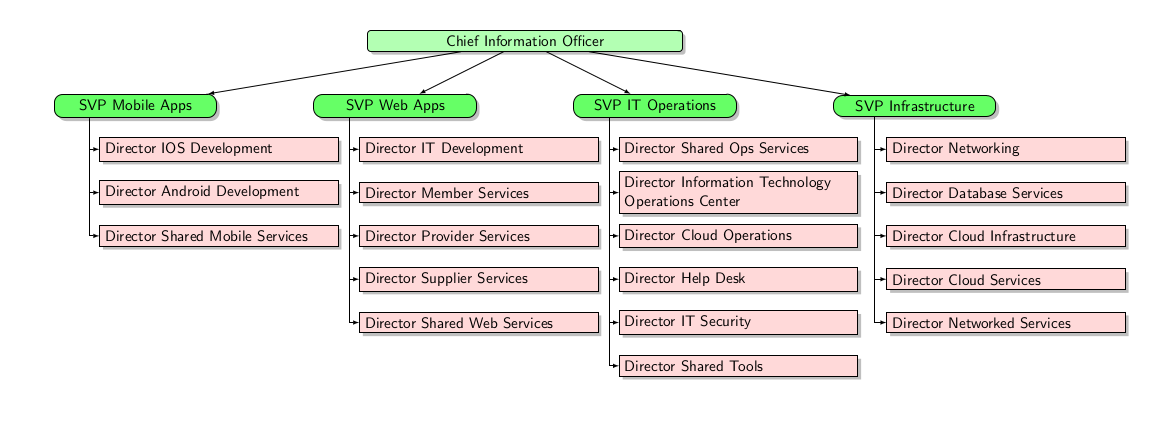
\includegraphics[width=.9\linewidth]{./diag1.png}
\caption{Initial Reporting Structure}
\end{figure}

This division of operations and development impacts the broader interactions. As it creates silos of where different considerations are the primary consideration for decision making. The development teams are guided by governance considerations where policy impacts development standards, whereas the operations teams are guided by service management procedures. While these procedures should ultimately be tied to policy, they are rarely, if ever, audited for policy compliance. The resulting structure is disjointed and segmented as seen in figure 2.

\begin{figure}[htbp]
\centering
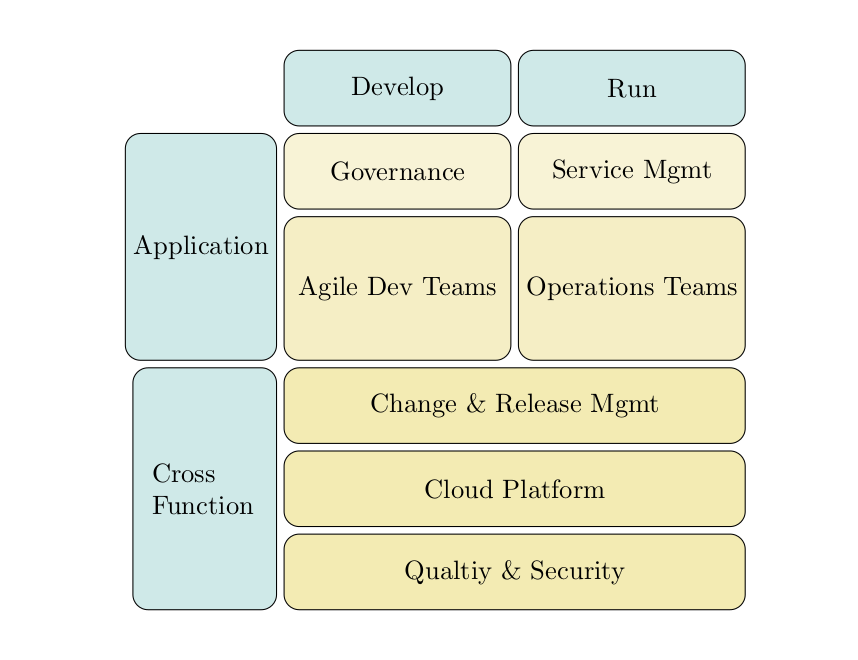
\includegraphics[width=.9\linewidth]{./diag2.png}
\caption{Traditional Silo Segmented Operations}
\end{figure}


This lack of ultimate support for the end users is seen in the initial state of the systems. While penalties exist for instability in the environment, the initial state of the client site was such that over the last 3 years the SLA of 99.9\% availability was missed more than a dozen times. Further, the actual causes of the instability in the environment remain largely unchanged year over year. The development teams are induced and bonused on the introduction of features, not on the stability of the environment after the introduction of those features. The Information Technology Operations Center ITOC teams are bonused on the closure rate of incidents, not on if the development teams or infrastructure teams take up stories related to improving stability and implementing them. This is a classic example of policy and organizational structure coming together to create a moral hazard \citep{depersioWhatAreExamples}. Each party is given incentives to ignore problems that bears an economic impact upon the broader company.

The overall result is both a low compliance to internal policy and a low concern for user experience. For example, of all Severity 1 tickets over the past year, only 39\% had a root cause analysis performed, and fewer than 20\% were closed within the policy mandated SLA. Further, while the company's stated SLA is 99.9\% Availability, it does not count scheduled maintenance windows into the availability calculation. The actual availability experienced by the user is much lower as seen in table 1.

\begin{table}[h]
\scriptsize
\begin{tabular}{@{}cccccc@{}}
\toprule
\textbf{MONTH} & \textbf{DAYS} & \textbf{HOURS} & \textbf{SCHEDULED DOWNTIME} & \textbf{ALLOWED OUTAGE} & \textbf{ACTUAL AVAILABILITY} \\ \midrule
Jan            & 31            & 744            & 20                          & 0.724                   & 97.215\%                     \\
Feb            & 28            & 672            & 20                          & 0.652                   & 96.927\%                     \\
Mar            & 31            & 744            & 40                          & 0.704                   & 94.529\%                     \\
Apr            & 30            & 720            & 20                          & 0.7                     & 97.125\%                     \\
May            & 31            & 744            & 20                          & 0.724                   & 97.215\%                     \\
Jun            & 30            & 720            & 32                          & 0.688                   & 95.460\%                     \\
Jul            & 31            & 744            & 32                          & 0.712                   & 95.603\%                     \\
Aug            & 31            & 744            & 32                          & 0.712                   & 95.603\%                     \\
Sep            & 30            & 720            & 32                          & 0.688                   & 95.460\%                     \\
Oct            & 31            & 744            & 40                          & 0.704                   & 94.529\%                     \\
Nov            & 30            & 720            & 32                          & 0.688                   & 95.460\%                     \\
Dec            & 31            & 744            & 32                          & 0.712                   & 95.603\%                     \\ \midrule
\textbf{TOTAL} & \textbf{365}  & \textbf{8760}  & \textbf{352}                & \textbf{8.408}          & \textbf{95.886\%}            \\
               &               &                &                             &                         &                              \\ \bottomrule
\end{tabular}
\end{table}

\section{INTERVENTIONS}
\label{sec:org68670ba}

In order to address the issues present, it was necessary to communicate effectively to leadership the interplay between organziational structure and policy and governance goals. Research has shown that organizational structure can strongly influence outcomes  \citep{soderstromOrganizationalStructureInteraction2020}. This impact includes the effectiveness of policy outcomes \citep{erhemjamtsCorporateSocialResponsibility2012}.

As the client's operational goals for a high quality environment sustaining a 99.9\% availability target were not being met, even with significant scheduled maintenance windows included, it is clear that the disparate reward systems in place for operations and development were creating problems that could not be adequately addressed by policy alone. To this end, organizational re-alignment was necessary to meet the policy goals of the organization.

The new organizational structure is much flatter. As there are inherently larger budgets at play, and greater number of direct reports, the titles are adjusted accordingly as in Figure 3.

\begin{figure}[htbp]
\centering
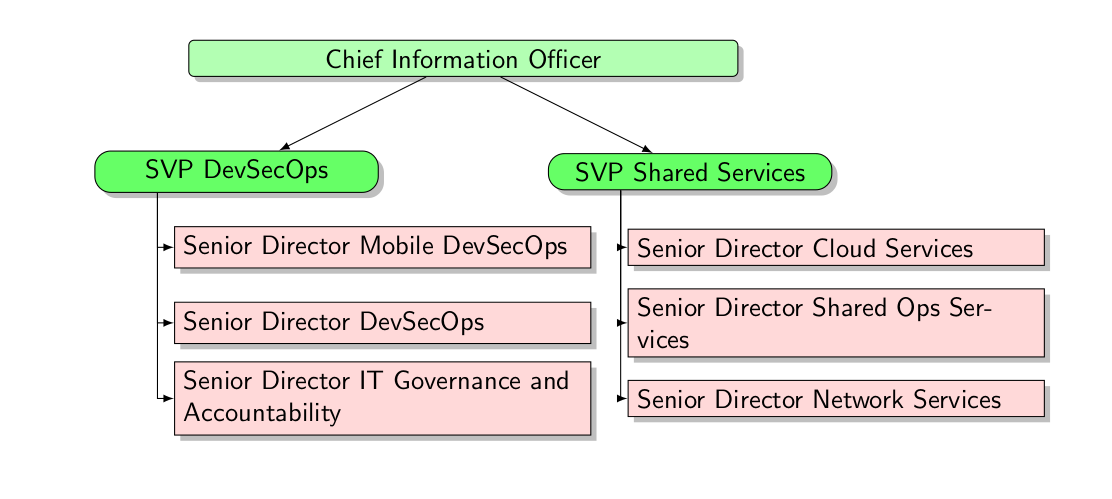
\includegraphics[width=.9\linewidth]{./diag3.png}
\caption{New Reporting Structure}
\end{figure}

Under each of the Senior directors exists a set of DevSecOps agile teams that are responsible for operating and development of their products. These product teams are headed by product managers responsible for understanding user needs. This structure ensures that the same team is responsible and accountable for both the development of new features and functionality and the support of the operational continuous running of the produced product in a secure manner.

The resulting shift in responsibilities moves to a single silo model as in Figure 4.

\begin{figure}[htbp]
\centering
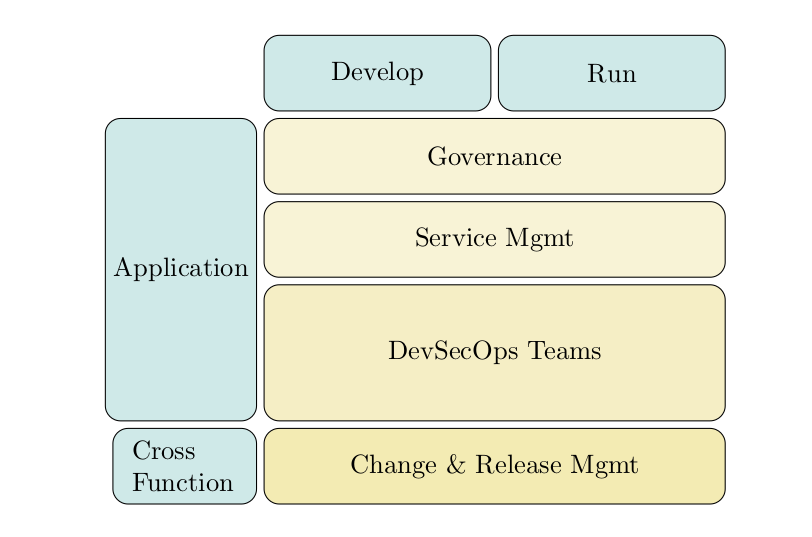
\includegraphics[width=.9\linewidth]{./diag4.png}
\caption{DevSecOps}
\end{figure}

This single silo of responsibility with a much shorter communications distance between any two teams ensures two significant outcomes. First, by increasing substantially the leadership scope of responsibilities, it forces leaders to delegate decision making further down into the organization, closer to the source of problems. This enhances employee empowerment which, when combined with adequate controls and training has been shown to substantially improve organizational performance  \citep{bairdRelationshipEnablingUse2018,al-omariRoleEmpowermentImproving2020}. Second, by making the same team responsible for both operations and development, and thus subject to direct governance controls as well as service management procedures, compliance to policies will be enhanced while at the same time making the team have to bear the burden of any quality defects introduced into the production environment. Further, this method has been shown to enhance both user satisfaction and employee satisfaction \citep[Sec. 4.3]{altContinuousInnovationDevOps} .

In addition to the organizational change, a significant policy change was implemented. The new policy moved to tracking all outages against an error budget initially calibrated to 1.5\% for the year. This meant that all downtime for the user would be tracked as equal, and the teams would have to take into account the impact of defects in production on their release schedule. When a product is stable, the teams can release more features more frequently, as there is room to introduce more instability into the environment. When there are more outages, then the teams need to cease development on new features and focus on restoring stability so that they can accumulate the error budget necessary to introduce the planned features. This completely eliminates all contention between operations and development as there is a single metric to guide the team as to if they can introduce an outage -- the user's experience of availability.

\section{Results}
\label{sec:orgf049c22}

As a result of the above changes, after 6 months in the new operating model the organization had reached a point where several key observations where made. First, there was much stronger policy compliance with reporting of incident data. While previously only 39\% of severity 1 tickets had a root cause analysis performed, over the ensuing 6 months since the change 86\% of severity 1 tickets have had root cause analysis performed. While previously the operations teams only closed 20\% of severity 1 tickets within SLA, in the last 6 months since these changes 54\% of severity tickets have made SLA.

In addition, the rate at which new features are being added to the production environment has increased roughly 45\% since the structural change. A change the employees have, through unstructured interviews, attributed to the ability to ``just go talk to the people they need to talk with'' in this new model.

Further, employees report much increased job satisfaction with the new structure.

There have been some difficulties to overcome. Senior leadership continues to express concern that they dislike feeling as though too many decisions are being made without their input or consultation. An indication that they are having some difficulty adjusting to the shift from a command-control structure to a more collaborative structure. However, they are quick to admit that the results with regards to incident management are exceptional.

Overall, it this appears to be a solid case study demonstrating that DevSecOps is a fitting option for a SME financial institution struggling with problematic IT incident policy compliance.



\newpage
\section*{REFERENCES}
\label{sec:org47bf538}
\printbibliography[heading=none]
\end{document}
